\chapter{Aircraft System Identification from Minimal Sensor Data}
\label{chap:aircraft_sysid}

\begin{quote}
    \emph{This chapter includes content from the author's prior publication} \cite{sharpe_physicsinformed_2024}.
\end{quote}

This chapter presents a system-identification-like process for estimating an aircraft's aerodynamic and propulsive performance characteristics from minimal flight data. The method is based on a physics-informed regression approach, which uses an unsteady physics model of the aircraft's dynamics to constrain the regression problem. The method is demonstrated on a flight test dataset collected from a small electric aircraft. The results show that the method is able to estimate the aircraft's power curve, aerodynamic polar, and propulsive efficiency curve with surprisingly high accuracy given limited data. In addition, we show that bootstrapped uncertainty estimates can be obtained for these performance curves using this method.

A related additional contribution is a new method for estimating the statistical properties of the noise component of a noisy signal, only using the noisy observations themselves. This relies on certain common assumptions about the noise-generating process, such as spectral separation between the true signal and the noise. Noise is isolated by repeated numerical differentiation, which is shown to be stable in numerical experiment and on application to actual flight data. An example implementation of this noise variance estimator is given and shown to be convergent to the true noise variance in numerical experiment. Higher-order implementations of this estimator are also presented and shown to isolate the noise accurately even when the underlying true signal is quite close to the Nyquist frequency.


\section{Introduction}

A primary goal of a new aircraft's initial flight test campaign is to experimentally determine the aircraft's aerodynamic and propulsive performance characteristics. The desired outputs of this process typically include:

\begin{enumerate}
    \item The aircraft's power curve, which gives the required power to maintain level flight as a function of airspeed.
    \item The aircraft's $C_L$-$C_D$ aerodynamic polar. This gives the relationship between the aircraft's lift and drag coefficients as angle of attack is varied, representing the locus of possible aerodynamic operating points.
    \item The aircraft's propulsive efficiency curve, which yields the overall propulsive efficiency, typically as a function of throttle setting and/or propeller advance ratio (if relevant).
\end{enumerate}

All three of these results represent sweeps through the aircraft's flight envelope, varying the aircraft's airspeed, pitch trim setting, and throttle setting, and measuring the resulting lift, drag, and power required.

\subsection{Traditional Flight Measurement Methods and Limitations}

Typically, these performance outputs are obtained by performing an extensive campaign of careful, controlled flight experiments at quasi-steady flight conditions.

For example, the aerodynamic polar is commonly measured by performing a series of long, steady power-off glides at different airspeeds, thus isolating the effect of propulsive power. (If the aircraft is propeller-driven, propeller windmilling drag can also be estimated and calibrated out for improved accuracy, although this introduces significant additional uncertainty.) An implicit assumption here is that pitch trim is adjusted to maintain these airspeeds. The glide ratio (or equivalently, if local airmass motion and airspeed changes are calibrated out, the $L/D$) is then measured at a given airspeed by using a simple two-point finite-difference between the beginning and end of the glide:

$$(L/D) = \frac{h(t_1) - h(t_2)}{U \cdot (t_2 - t_1)}$$

where $h(t)$ represents the altitude at time $t$, $U$ represents the airspeed, and $t_1$ and $t_2$ are the beginning- and end-times of the glide. The drag is then computed as $D = W / (L/D)$, and $C_L$ and $C_D$ can be nondimensionalized from here.

For aerodynamically-efficient aircraft with high $L/D$ ratios (such as sailplanes), using this strategy without calibration leads to substantial error due to airmass motion (e.g., thermals, ridge lift) and airspeed changes. Instead, another common strategy for estimating aerodynamic polars during flight testing is to fly these power-off glides along with a wingman aircraft. This wingman aircraft flies the same power-off glide as the test aircraft, at the same airspeed, with the same starting altitude, and in the same vicinity. The wingman aircraft is assumed to have a known aerodynamic polar, and hence the difference in altitude between the two aircraft at the end of a glide segment can be used to estimate the test aircraft's aerodynamic polar. This approach calibrates out the effect of local airmass motion on the measured glide ratio.

More extreme strategies have also been implemented to measure the aerodynamic performance curve. For example, the glide ratio of the P-51 fighter aircraft was allegedly measured by removing the propeller, towing it aloft, and gliding it down. This removes the error associated with estimating propeller windmilling drag, but this is obviously an onerous, expensive, and potentially less-safe procedure to include in a flight test campaign.

Full-scale wind tunnel testing is another possible method for estimating the aerodynamic polar of the as-built aircraft, although this is similarly expensive and time-consuming, rendering it infeasible for most aircraft development programs. Scale models in wind tunnels as well as CFD simulation can also provide useful aerodynamic estimates, but these results can differ significantly from the aerodynamics of real as-built aircraft. For example, Hoerner \cite{hoerner_fluiddynamic_1965} gives a pathological example of the Messerschmitt Bf 109 fighter aircraft, where roughly \emph{half of the drag of the as-built aircraft} is attributable to components that are typically de-featured in modern computational analysis\footnote{e.g., rivets, sheet metal gaps, control surface gaps \& hinges, engine and radiator thermal effects, inlet flow distortion, antennae, sensors, lights, guns, holes for ventilation and cooling, etc.}. This Bf 109 case likely has an unusually-high number of such protuberances, but even for modern aircraft, the drag of the as-built aircraft can differ significantly from computational estimates or small-scale wind tunnel testing. This motivates flight-test-based aerodynamic polar characterization.

Like the aerodynamic polar, the power curve is also often measured by flying in steady flight segments at various airspeeds. For each airspeed, level flight is held with power and pitch trim adjusted as needed for stabilized cruise. The required input power to the propulsion system $P_{\rm in}$ is then measured. In a conventionally-fueled airplane, this can be computed using the fuel flow rate at a given throttle setting (read off the panel via a fuel flow meter) and the specific energy of the fuel, or indirectly from the engine RPM depending on the powerplant data available. For an electric airplane, it can be computed as the product of battery current and voltage, which are readily available. This procedure is then repeated for a variety of airspeeds, and the resulting power curve is plotted.

The propulsive efficiency can be roughly estimated based on these experiments as well. One possible procedure is as follows:

\begin{enumerate}
    \item The input power to the propulsion system $P_{\rm in}$ is measured, as above.
    \item We observe the steady-state climb/sink rate of the aircraft at this throttle setting and we compare this to the power-off sink rate. The difference between these two sink rates represents the thrust power done by the propulsion system. The thrust power (or ``air power'') can be computed as:

    $$P_{\rm thrust}=T \cdot U = m g \left( \frac{dh}{dt}\Big |_\text{power on} - \frac{dh}{dt}\Big |_\text{power off} \right)$$

    \item Then, we can compute the propulsive efficiency as the ratio of the input power to the air power:

    $$\eta_{\rm propulsive} = \frac{P_{\rm thrust}}{P_{\rm in}}$$

\end{enumerate}

These traditional methods for measuring aerodynamic and propulsive performance have several limitations. The biggest limitation by far is that they require vast amounts of flight time to obtain a sufficient number of data points to characterize the aircraft's performance.

Furthermore, the aircraft must be flown at precisely-controlled conditions. Traditional methods are not well-suited to estimating the performance of an aircraft that is not in steady flight -- in the methods described here, only steady data (e.g., a stabilized glide or cruise) can be used. For example, data recorded during an aircraft's climb or descent to flight test altitude is discarded, which is wasteful; ideally, every single second of data should contribute to refining our estimate of the aircraft's performance. This requirement to maintain steady conditions can be frustrating and tedious for the pilot to maintain, and it can also be dangerous if the aircraft is flown for an extended duration at conditions that are close to the edge of the flight envelope (e.g., behind the power curve on a not-yet-characterized experimental airplane).

Traditional methods also make no direct estimate of sensor noise (and hence, uncertainty) -- data is collected and averaged until the experimenter is satisfied that the data is ``good enough''. This is a subjective process that leaves it difficult to quantify the uncertainty in the resulting performance estimates.

Nevertheless, the methodology described here provides a useful existence proof that airplane performance curves are fundamentally observable (and hence, able to be recovered) given airspeed, altitude, and power data of sufficiently varied flight. A primary goal of this chapter is to develop a methodology that can estimate these performance curves from a much smaller amount of flight data, which would decrease the cost and intentionality required to obtain these performance estimates.

\subsection{Inference-Based Flight Data Reconstruction Methods}

We propose a method of estimating these performance characteristics that views the aircraft flight test as a data-generating process, from which we can infer performance relationships. Figure \ref{fig:overall_procedure} broadly illustrates the toolchain for performance reconstruction that represents this chapter's central contribution. This approach contrasts with traditional methods, which view flight testing as a process of pure measurement, based only on analyzing the data itself. This distinction manifests in a few ways, each of which recognizes that we have process- or domain-specific information that collapses the possible solution space of possible performance models:

Firstly, with certain reasonable assumptions about the sensor noise characteristics, the data itself can reveal a surprisingly large amount of information about the sensor noise. Essentially, this involves using the data to estimate the ``trustworthiness'' \emph{of the data itself}, a process described more fully in Section \ref{subsec:optimal_sensor_data_reconstruction}. One contribution of this chapter is a new cross-validation-like approach for estimating the sensor noise using only the properties of the data itself. This allows cleaner raw data inputs to the subsequent performance analysis toolchain that we develop, ultimately resulting in more accurate performance estimates and aiding uncertainty quantification. In Figure \ref{fig:overall_procedure}, this is represented by the separation of sensor data into its signal and noise components.

We also know certain characteristics of the aircraft's performance curve based on first-principles physics, which can further increase the effective information density and our resulting performance estimates. Another way to think about this is that the function space of performance curves is restricted to functions that generally follow first-principles physics, allowing us to reduce uncertainty on these resulting inferred relations. For example, we know that the true state of the aircraft must follow invariants from Newtonian physics (e.g., conservation of energy). Likewise, propulsive efficiency is a bounded function that must not exceed unity to be physically plausible. Embedding these constraints and invariants from physics reduces the number of unknowns, enabling more robust correction for unsteady effects. This is described in Section \ref{sec:physics_based_corrections}.

Finally, there are characteristics about performance relations that we can be embedded from domain-specific expertise. Even for models that do not have simple, closed-form invariants, we almost always have some priors (i.e., informed guesses) about how performance parameters should be related - model structure. For example, we know that the aircraft's drag coefficient will primarily be a function of lift coefficient, and the general shape of this function is known. Similarly, we know that the propulsive efficiency will largely be a function of advance ratio, and the advance ratio can be inferred from the airspeed, input power, and first-order physics. Incorporation of these physics-based performance models embeds our physical understanding of the aircraft system into the estimation process, improving accuracy. For this reason, we term the performance reconstruction methodology described in this work a ``physics-informed'' approach.

The example given in the subsequent sections is for a small electric-driven propeller aircraft, although the methodology is applicable to any aircraft type. Some considerations for applying this methodology to other aircraft types are discussed in Section \ref{sec:sysid_conclusion}.

\begin{figure}[h]
    \centering
    \ifdraft{}{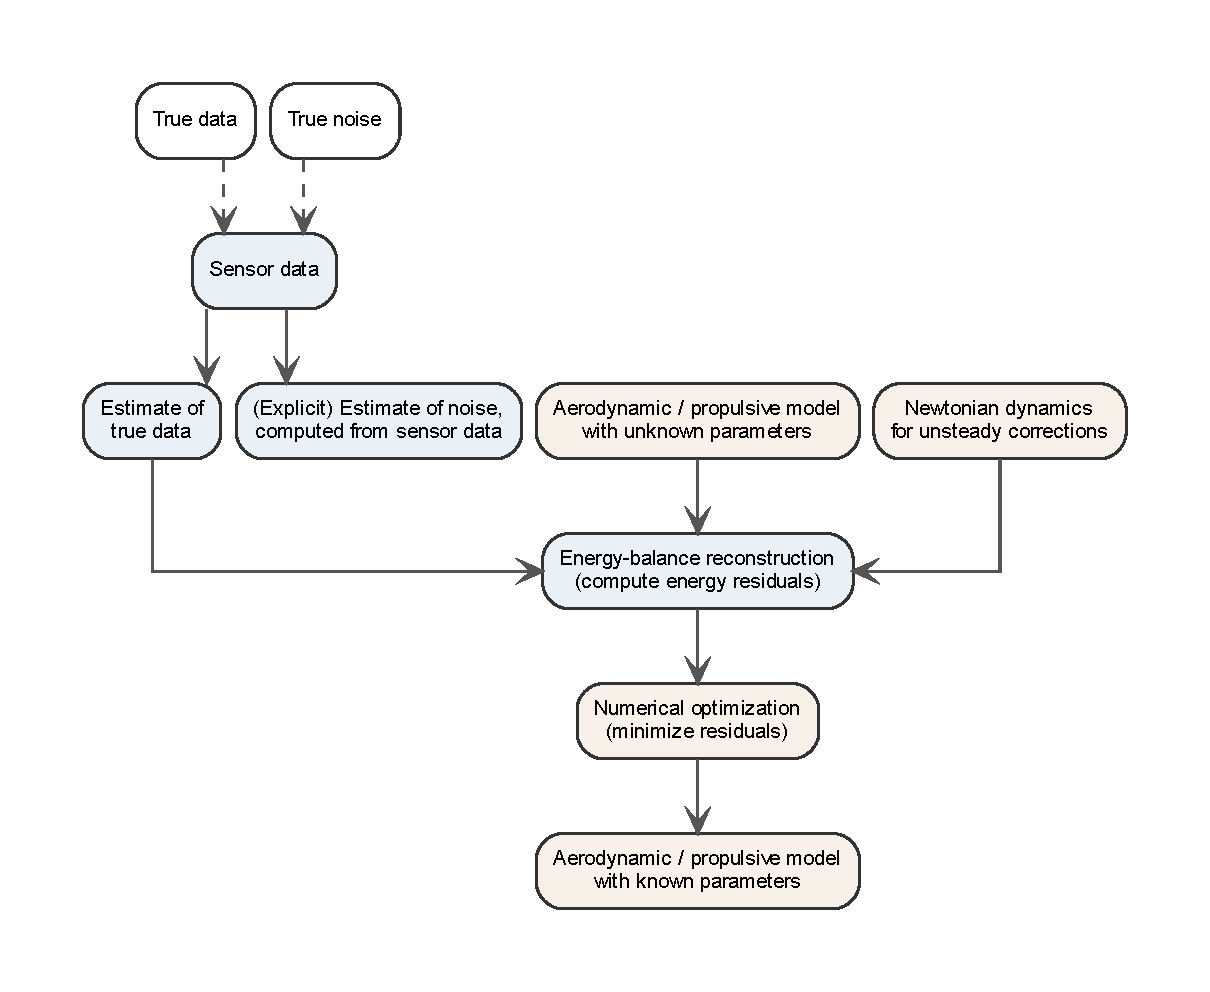
\includegraphics[width=\textwidth, trim=1cm 1cm 1cm 1cm,clip=true]{../figures/aircraft_sysid/overall_procedure}}
    \caption{Process for inference-based performance reconstruction from flight data}
    \label{fig:overall_procedure}
\end{figure}


\section{A Minimal Flight Test Dataset}

To illustrate our proposed flight test data analysis procedure, this manuscript will use example data from a flight test conducted during MIT 16.821: Flight Vehicle Development, a senior-level aircraft design/build/fly capstone course at MIT AeroAstro. The flown aircraft, named \emph{Solar Surfer}, is a remote-controlled solar-electric seaplane design with a 14-foot wingspan. The as-flown all-up mass is 9.4 kg.

General specifications of the aircraft can be found in the early design drawing that is reproduced in Appendix \ref{sec:solar_surfer_drawing}. While this drawing does not reflect as-built weights or various planform adjustments that were made during preliminary design and construction, the overall configuration and performance numbers are representative of the aircraft that was flown.

\subsection{Flight Test Campaign}

The aircraft was flown in the vicinity of the Charles River basin near Cambridge, MA. Five tests were conducted on the morning of May 3, 2023, of which two were airborne flight tests. The final airborne flight test lasted approximately 260 seconds (4.3 minutes), beginning and ending with a successful water takeoff and landing. Figure \ref{fig:solar_surfer_flight} depicts a still image of the aircraft in flight. A simple racetrack-like pattern was flown, as shown in Figure \ref{fig:solar_surfer_track}. Winds were calm at roughly 1.5 m/s from the south.

\begin{figure}[h]
    \centering
    \begin{subfigure}[b]{0.45\textwidth}
        \ifdraft{}{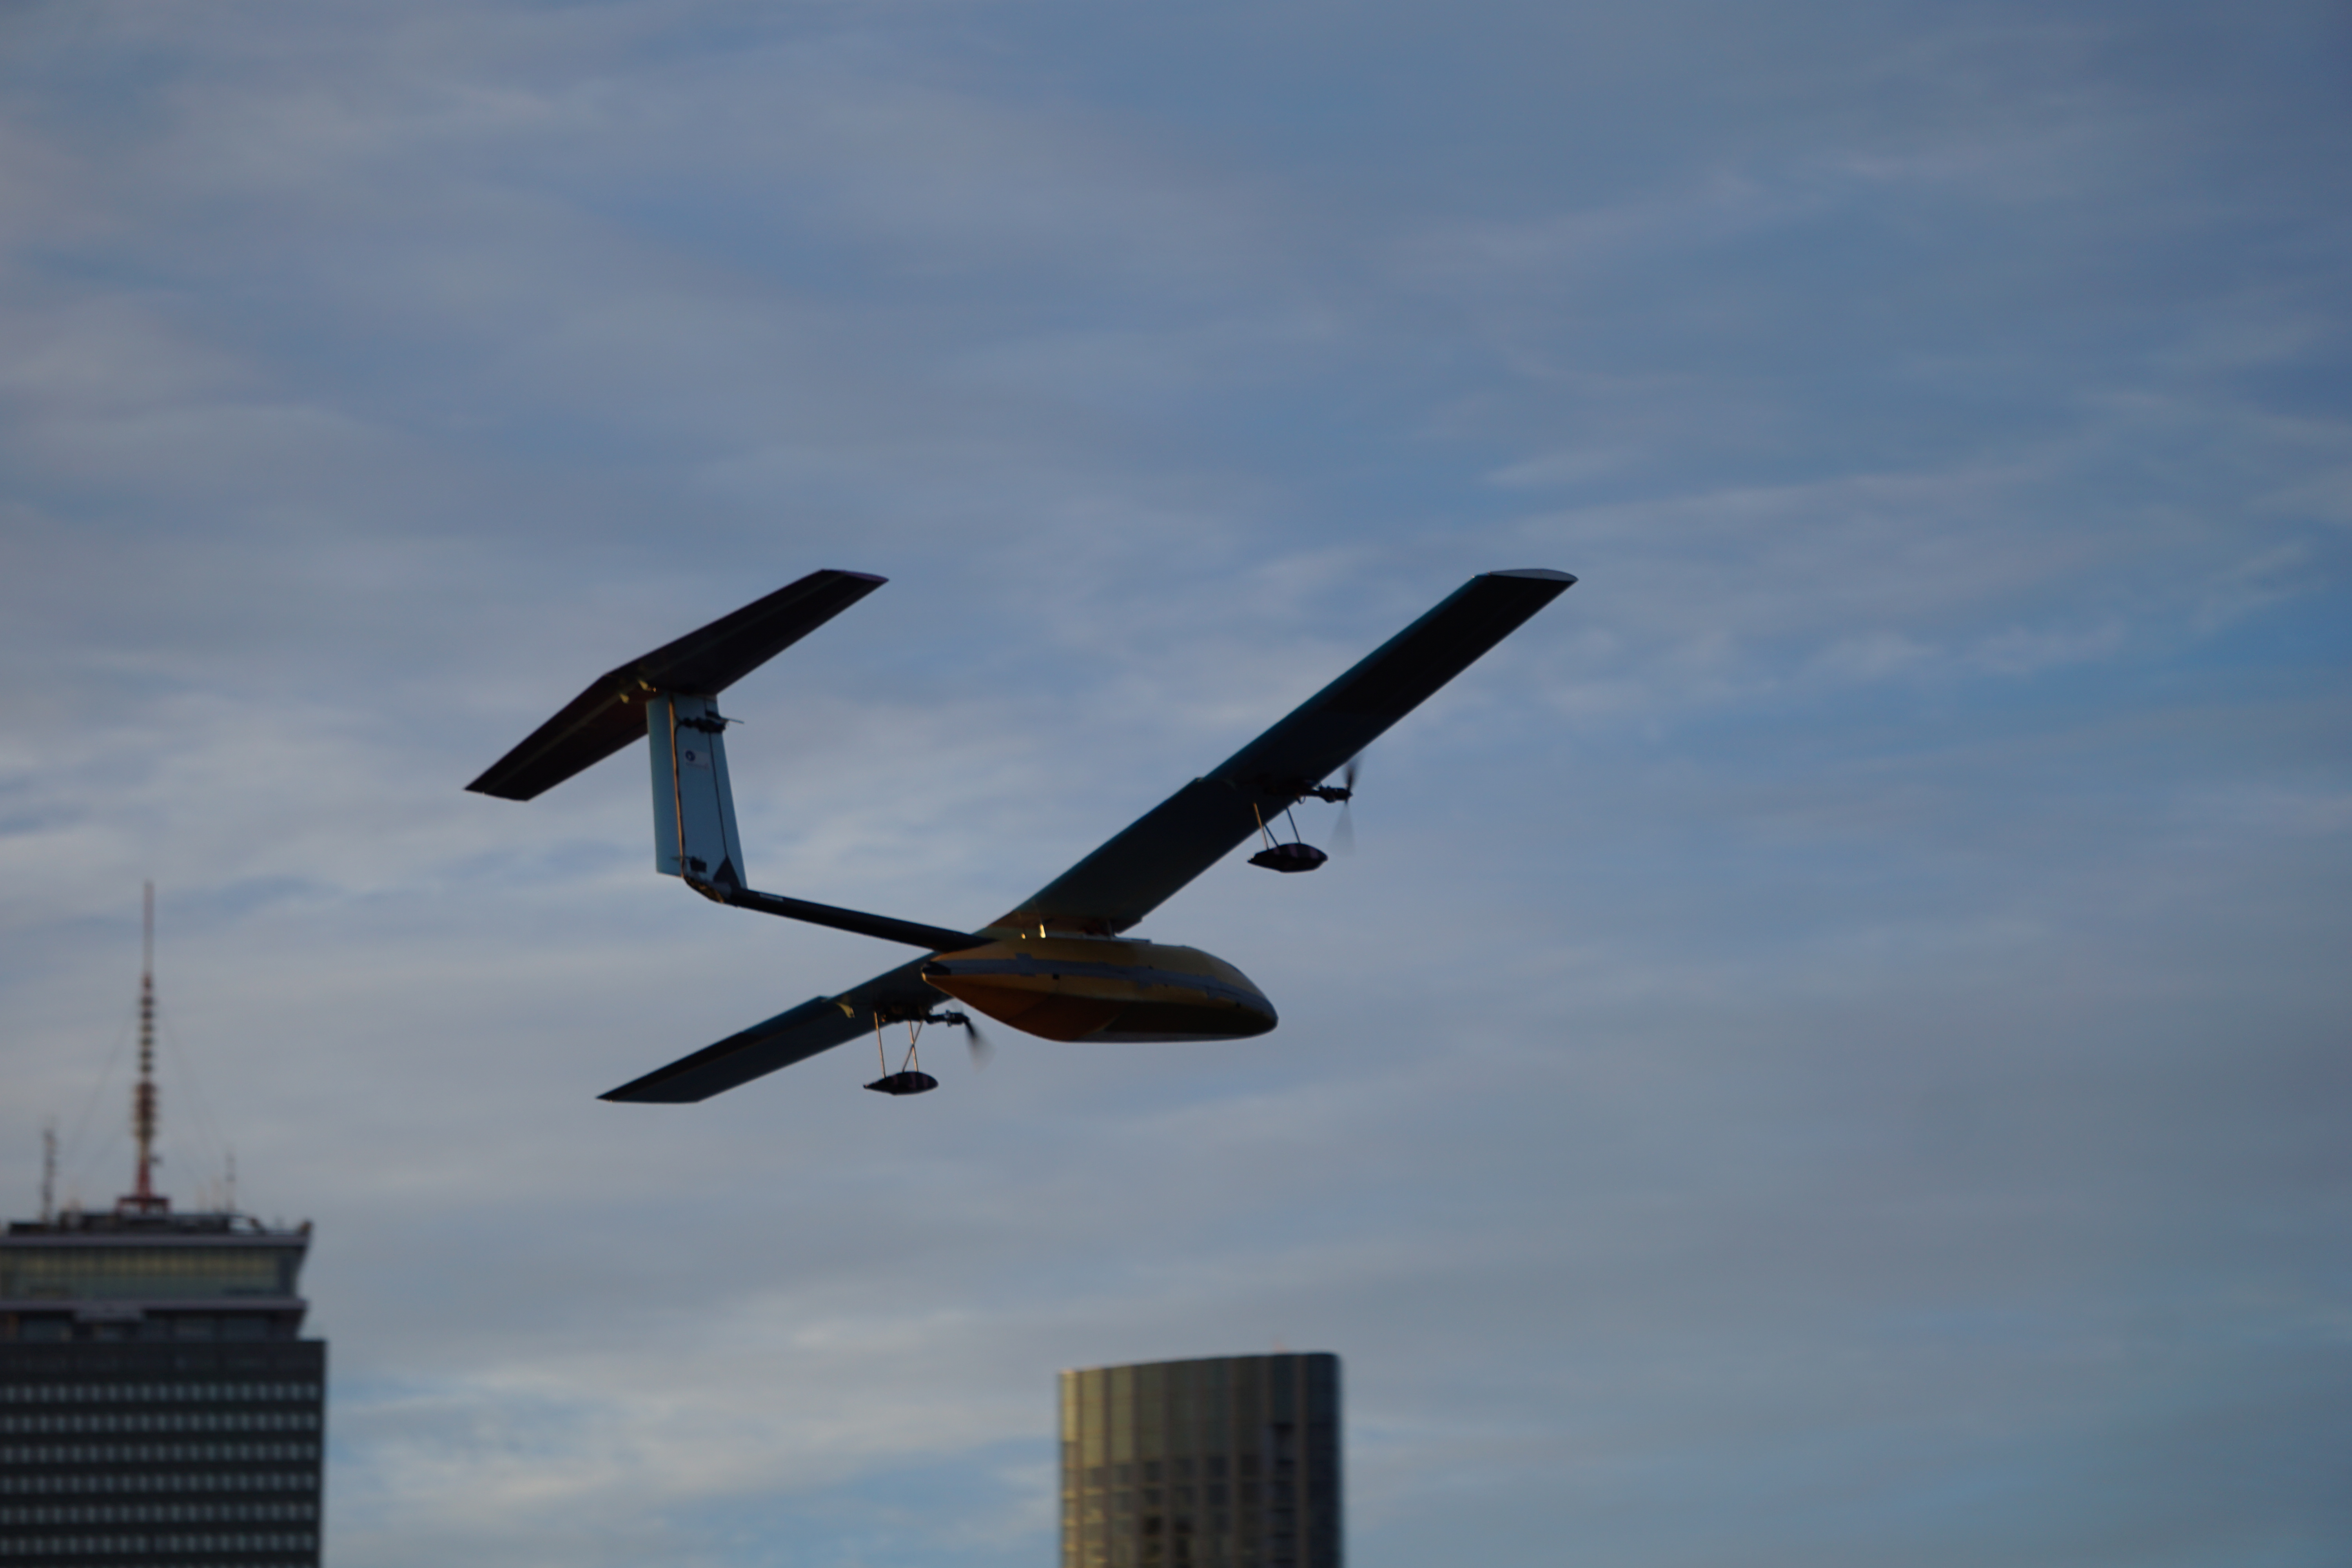
\includegraphics[width=\textwidth]{../figures/aircraft_sysid/Flight1_02549.JPG}}
        \caption{\emph{Solar Surfer} in flight}
        \label{fig:solar_surfer_flight}
    \end{subfigure}
    \hfill
    \begin{subfigure}[b]{0.511\textwidth}
        \ifdraft{}{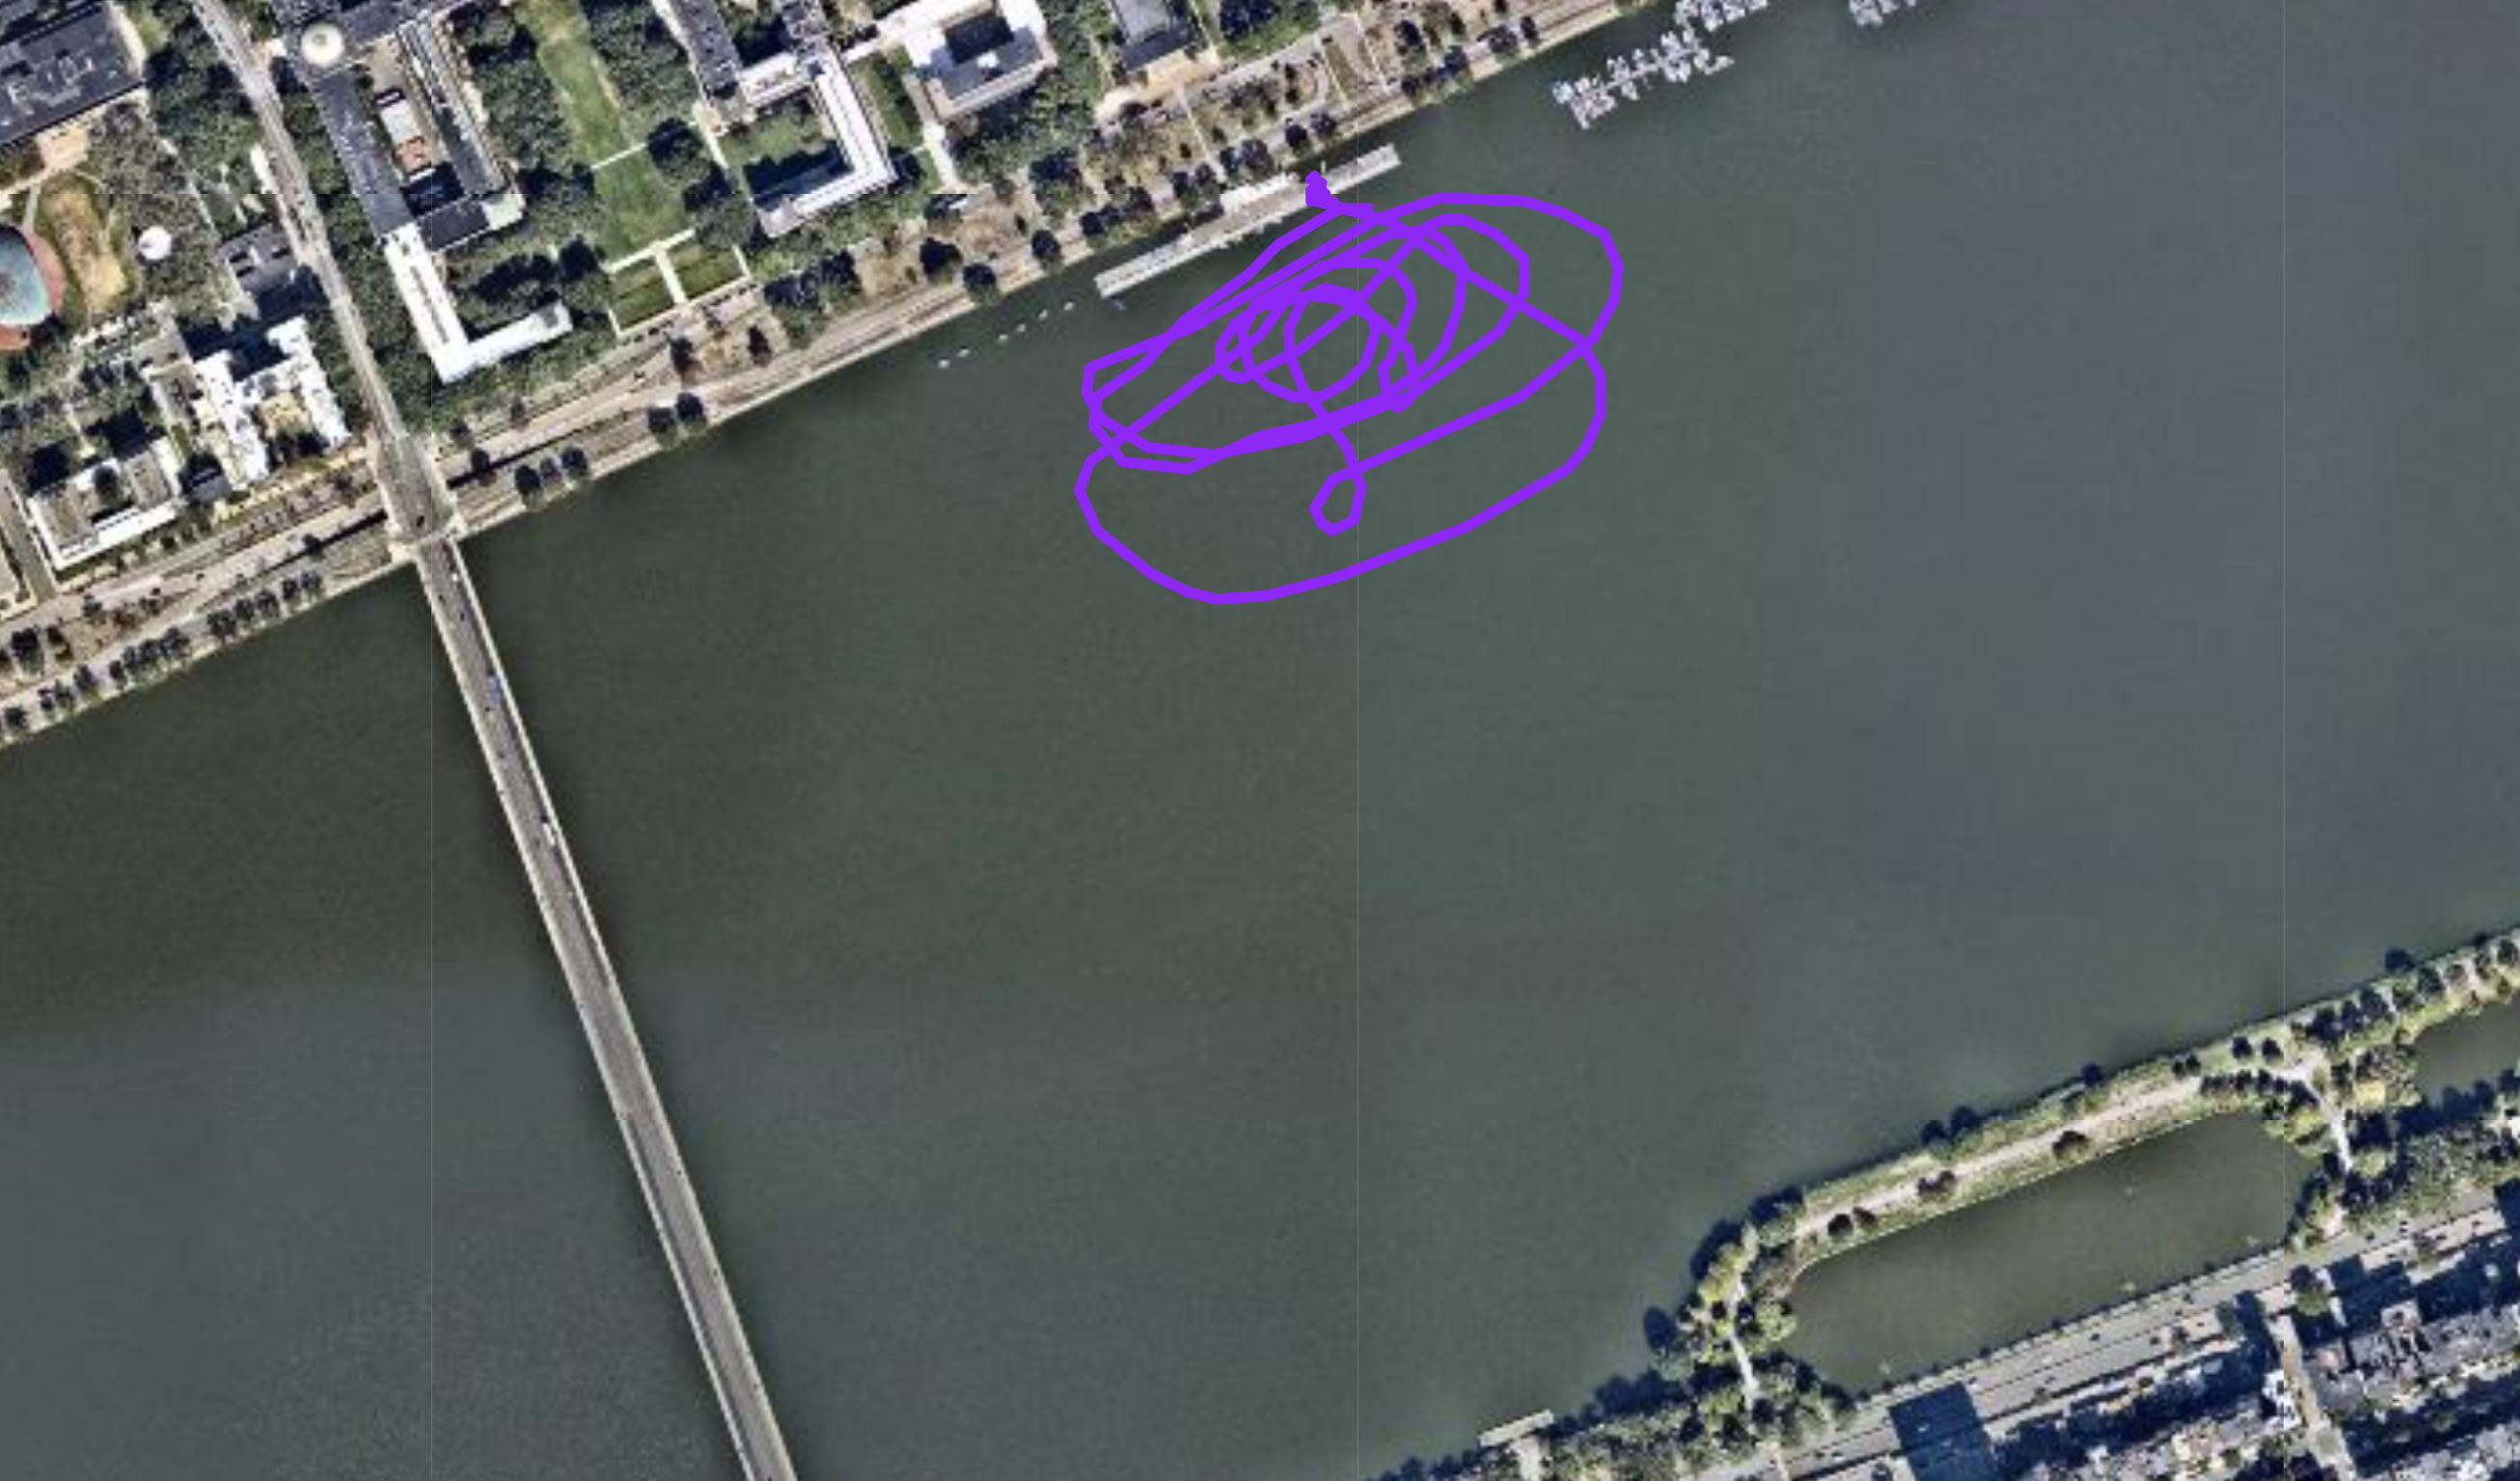
\includegraphics[width=\textwidth]{../figures/aircraft_sysid/flight3-circuit}}
        \caption{Recorded GPS ground track during test flight}
        \label{fig:solar_surfer_track}
    \end{subfigure}
    \caption{\emph{Solar Surfer} aircraft test flight}
    \label{fig:solar_surfer_aircraft}
\end{figure}

Figure \ref{fig:raw_flight_data} illustrates the subset of the raw sensor data during flight that will be used for performance reconstruction. Overall, the data is reasonable, and we can clearly identify takeoff and landing by the strong increase in barometric altimeter noise near $t=0\ \rm sec$ and $t=263\ \rm sec$. We can also identify several distinct flight phases, such as a high-speed pass near $t=150\ \rm sec$ and gliding periods near $t=40\ \rm sec$, $t=210\ \rm sec$, and $t=250\ \rm sec$.

\begin{figure}[h]
    \centering
    \ifdraft{}{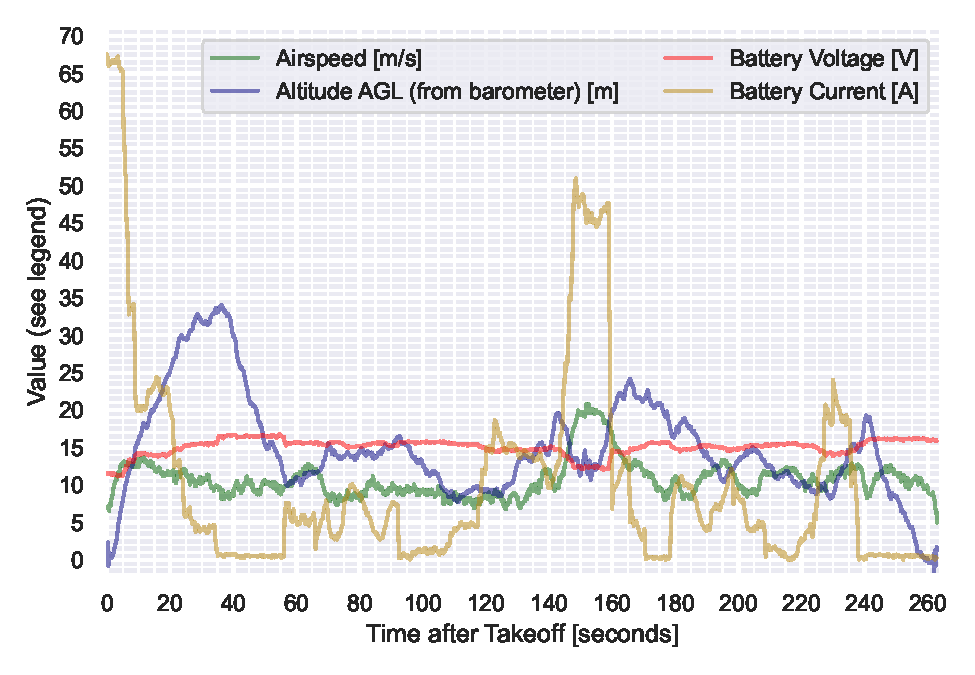
\includegraphics[width=\textwidth]{../figures/aircraft_sysid/flight_raw_data}}
    \caption{Raw sensor data from \emph{Solar Surfer} aircraft test flight}
    \label{fig:raw_flight_data}
\end{figure}

Summary statistics of this data are given in Table \ref{tab:aircraft_stats}.

\begin{table}[h]
    \centering
    \caption{Summary statistics of raw sensor data from \emph{Solar Surfer} aircraft test flight. Based on 1,315 samples per measured quantity.}
    \begin{tabular}{lcccc}
        \toprule
        Description   & Airspeed [m/s] & Altitude AGL [m] & Voltage [V] & Current [A] \\ \midrule
        Mean          & 10.8           & 16.4             & 15.05       & 10.31       \\
        Standard Dev. & 2.52           & 6.81             & 1.08        & 13.73       \\
        Min           & 5.0            & 0                & 11.13       & 0.00        \\
        25\%          & 9.1            & 12.3             & 14.69       & 0.94        \\
        50\%          & 10.3           & 15.4             & 15.28       & 5.25        \\
        75\%          & 11.7           & 19.3             & 15.67       & 13.28       \\
        Max           & 20.9           & 35.6             & 16.77       & 67.53       \\ \bottomrule
    \end{tabular}
    \label{tab:aircraft_stats}
\end{table}

However, there are two primary problems with the data we have. Firstly, all the data sources, and in particular the airspeed sensor, yield noisy measurements. The unsteady corrections that we will later implement require taking the derivative of this data; this is a problem because taking the derivative of noisy data tends to amplify the noise further.

Secondly, the total amount of data is extremely limited, both in duration and sample rate. For example, there are only 1,315 data points \emph{in total} for each of the plotted sensor traces. After eliminating noise (which effectively acts as a low-pass filter on our data, as noise tends to be relatively high-frequency), the effective amount of information we have from the sensors is quite limited. While traditional methods might be able to extract general aircraft flight performance based on this quantity of data (i.e., average required power over the flight), a detailed airspeed-based power curve is not typically achievable with such limited data.

Consider that even the most sophisticated techniques for system identification via statistical inference require the system to be observable in some form - no amount of math can recover a signal that is simply not present in the data. This is difficult, because after noise removal, the data really no more than perhaps a half-dozen ``system excitations'' from which we can infer aircraft performance. For these reasons, this dataset makes a good example case for what kinds of flight data reconstruction are possible with very limited, noisy data using statistical inference techniques and corrections from unsteady flight physics.

\subsection{Naive Estimation of Power Curve}

The most straightforward approach to estimating the aircraft's power curve is to simply cross-plot the airspeed and electrical power throughout the flight, and then to fit a curve to it.

Figure \ref{fig:power_curve_naive} quickly illustrates the infeasibility of this approach. While a general trend is somewhat apparent (higher airspeeds yield higher power draw), the uncorrected data has far too much unexplained variation and noise to make any believable conclusions about the shape of the power curve.

Figure \ref{fig:power_curve_naive} also demonstrates the pitfalls of naive curve-fitting in the absence of any kind of physics-based model structure. Perhaps the most severe of these is the extrapolation to physically-impossible conclusions. For example, the naive linear fit shown in blue would imply that the power draw at zero airspeed is negative, which is clearly impossible. The naive cubic fit shown in red initially appears more reasonable, although it too makes erroneous conclusions: it implies that beyond $20\ \rm m/s$, the power draw decreases with increasing airspeed. Clearly, our intuitions about what the ``correct'' model would look are not being incorporated into the curve-fitting process, and hence we are leaving information on the table.

\begin{figure}[h]
    \centering
    \ifdraft{}{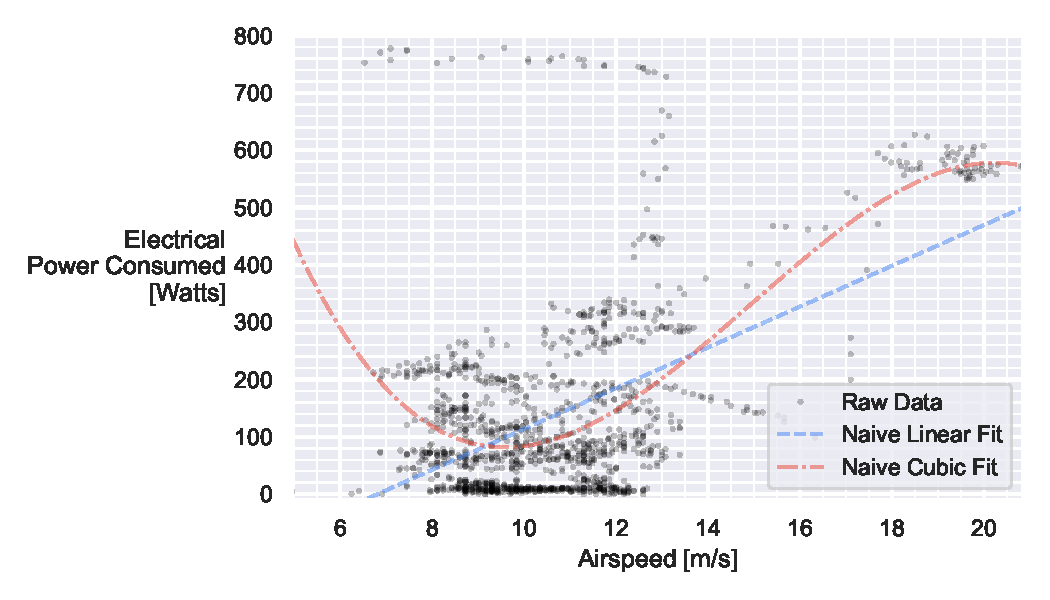
\includegraphics[width=\textwidth]{../figures/aircraft_sysid/power_polar_naive}}
    \caption{Raw uncorrected data for the power curve, with naive curve fitting to demonstrate the infeasibility of this approach. Uncorrected data exhibits high amounts of unexplained variance. Naive curve fits extrapolate to physically-impossible conclusions and do not capture uncertainty.}
    \label{fig:power_curve_naive}
\end{figure}


\section{Sensor Data Pre-Processing}

The first contribution here is to develop a means of pre-processing the sensor data to isolate noise; readers who are more interested in in physics-informed regression than uncertainty quantification may skip forward to Section \ref{sec:physics_based_corrections}. Traditionally, noise is removed by simple averaging; after this process is complete, any uncertainty in the data is typically not considered, and the average is regarded as the ground truth. This works fine for traditional steady analysis where there is a wealth of data that we can average over.

However cases where data is limited provide a strongly incentive to find a way to extract some amount of information from unsteady data. This is difficult because it forces us to directly deal with the sensor noise (and embed priors about the bias-variance tradeoff of data), rather than hand-waving it away by averaging.

As an illustrative example, imagine that we wish to reconstruct a \emph{truth} estimate of the airspeed from the example dataset. This truth value is not directly observable, although data from an associated airspeed sensor is. However, this sensor data has noise; hence, any attempt to reconstruct the truth value must adopt a strategy to separate the noise from the data.

However, there are (literally) an infinite number of possible strategies that one can use to do this noise removal, depending on our embedded assumptions about how sensor noise is entering our data-generating process. For example, consider three different possible state estimations of the vehicle's airspeed, as illustrated in Figure \ref{fig:under_over_fitting}.

\begin{figure}[h]
    \centering
    \ifdraft{}{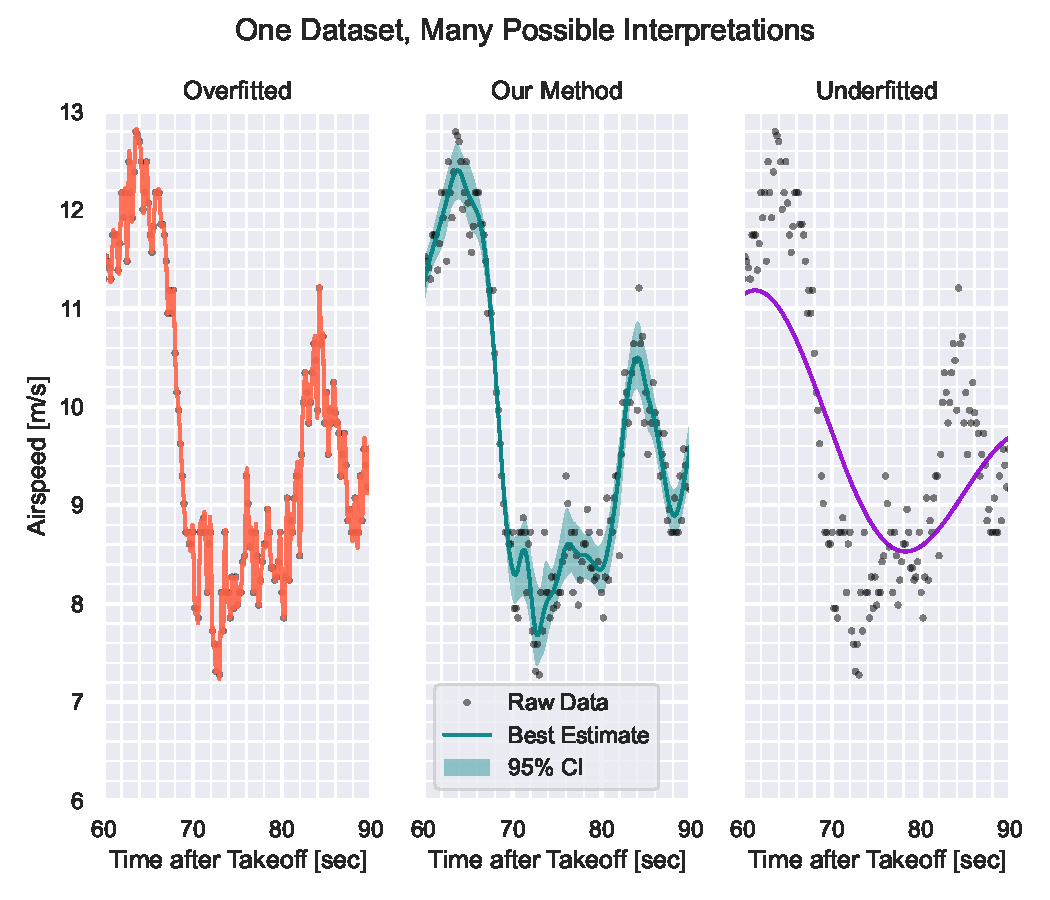
\includegraphics[width=\textwidth]{../figures/aircraft_sysid/under_over_fitting}}
    \caption{Three possible curves that could be used to estimate the true underlying state of the vehicle. Airspeed data, zoomed to $t \in (60, 90)$; a subset of Figure \ref{fig:raw_flight_data}. 95\% confidence interval (CI) of reconstruction shaded in middle plot.}
    \label{fig:under_over_fitting}
\end{figure}

Ultimately, all three charts in Figure \ref{fig:under_over_fitting} represent different interpretations of the ground truth based on the data. If we didn't have any more information about the problem, all three could be equally justifiable given the appropriate context—but, in fact, we do have more information, since we know this data originates from a physical system.

The chart on the left of Figure \ref{fig:under_over_fitting} is clearly overfitted (i.e., tracks the data too closely) based on engineering intuition. Essentially, we are assuming that each sample is the true data, and that each sample has no noise; hence, the ``truth'' curve exhibits extremely high variance (strong wiggles). There is no \emph{mathematical} reason why this interpretation can't be correct (it's theoretically possible that the sensor is giving perfect information), but of course, it is is \emph{physically} implausible for our system. If this interpretation were true, it would imply that the vehicle is achieving velocity-vector-aligned accelerations on the order of 2.4 G, which is not physically plausible given the onboard propulsion system.

The chart on the right of Figure \ref{fig:under_over_fitting} is clearly underfitted (i.e., tracks the data too slowly), as there are large regions where the estimator has a consistent bias (e.g., consistently too high or low) with respect to the underlying data. It might seem like there are no contexts where such an interpretation would be reasonable, but that is not necessarily the case. For example, if the sensor noise at each sample was not independent, but rather correlated with noise from the previous samples, we might not be able to rule out this interpretation of reality.

Of course, a quick glance at the three charts above would tell us ``the middle one looks about right'', although it's not immediately clear why.

\subsection{Optimal Sensor Data Reconstruction using Data-Driven Noise Estimates}
\label{subsec:optimal_sensor_data_reconstruction}

The key difference is that the middle chart embeds certain assumptions that we intuitively know about our data into its reconstruction. Specifically, the middle chart is an optimal reconstruction of the data assuming that:

\begin{itemize}
    \item The noise in each sample is independent (i.e., uncorrelated with previous samples) and normally-distributed
    \item The noise is unbiased (i.e., there are no systematic errors in the data, only random ones)
    \item The noise is homoscedastic (i.e., the standard deviation of the noise is constant across the entire dataset)
    \item The sample rate is significantly higher than the underlying dynamics of the system that we aim to recover (i.e., the system is ``slow'' relative to the sample rate), with this assumption quantified later in Section \ref{sec:sysid_first_order_noise_estimator}.
\end{itemize}

Under these assumptions above, the probabilistic properties of the noise reduce to a single parameter: the variance of the noise $\sigma^2_n$. Thus, by constructing an estimator for this statistic, we can recover the probability distribution of the noise and hence an optimal estimator of the data.

\subsubsection{Motivation for Finding the Variance of the Noise}

The variance of the noise is a useful quantity to estimate for several reasons. First, a probabilistic model of the sensor noise allows us to make optimal choices about the bias-variance tradeoff, armed with a rigorous definition of what optimal means here.

There is a second factor that motivates us to estimate the variance of the noise. Computing an optimal smoothing spline for a time-series dataset is a well-studied problem, but this process is greatly aided if we know the variance of the noise \cite{wahba}. So, if we can obtain an estimate of noise variance, we've done most of the work required to compute an optimal data reconstructor.

In an ideal world, we would estimate this variance of the noise by taking a large number of samples while the vehicle is at some fixed, steady, known condition. For example, to estimate the airspeed data noise, we might place the aircraft in a wind tunnel at some constant speed. If we ran that experiment for an extended duration, we would know that the true underlying data was constant, and hence any observed variance in the samples would be due to the variance of the sensor noise.

If we want to reconstruct data from unsteady measurement, however, we need to find a way to estimate the variance of the noise using the unsteady data itself, which is much more difficult.

\subsubsection{Initial Approach and a First-Order Data-Based Noise Estimator}
\label{sec:sysid_first_order_noise_estimator}

One way to do this is by assuming that the data is ``slow'' relative to the sample rate, while the noise remains white. If this is true, then subsequent samples will effectively have the same underlying truth value, but with noise drawn independently from the same underlying distribution.

Quantitatively, consider a scenario where the measured data $x(t)$ consists of a true signal $s(t)$ and noise $n(t)$:

$$x(t) = s(t) + n(t)$$

Assume the noise of the sample $n(t)$ is drawn from $\mathcal{N}(0, \sigma^2_n)$, with initially-unknown $\sigma_n$. Now, consider two discrete measurements taken at adjacent points in time $t_1$ and $t_2$:

\begin{align*}
    x(t_1) = s(t_1) + n(t_1) &&
    x(t_2) = s(t_2) + n(t_2)
\end{align*}

\noindent If $t_1 \approx t_2$ (as would be the case for subsequent samples), then $s(t_1) \approx s(t_2)$, contingent on the sample rate greatly exceeding the effective fastest frequency of the true signal. Hence:

$$x(t_2) - x(t_1) \approx n(t_2) - n(t_1)$$

In other words, the difference of two subsequent observed samples will be approximately equal to the difference of two independent draws from the same noise distribution. This means that we can estimate the variance of the noise by looking at the variance of the differences between subsequent samples. From the properties of the difference of two independent random normal variables, we can then say:

$$n(t_2) - n(t_1) \sim \mathcal{N}(0,\; 2\, \sigma^2_n)$$

\noindent where $\sigma^2_n$ is the variance of the sensor noise. So, the following is then approximately true:

$$x(t_2) - x(t_1) \sim \mathcal{N}(0,\; 2\, \sigma^2_n)$$

Therefore, taking the mean difference across all adjacent pairs of measured data $x(t)$ provides an unbiased estimator of $\sigma_n$, the variance of the noise:

\begin{equation}
    \sigma^2_n = \frac{1}{2 \cdot (N-1)} \sum_{i=1}^{N-1} \Big( x(t_{i+1}) - x(t_i) \Big)^2
    \label{eq:1st_order_noise_estimator}
\end{equation}

\noindent where $N$ is the number of samples in the dataset. We call this a \emph{first-order} noise estimator as it takes a first-order numerical derivative of the measured data.

\subsubsection{Numerical Demonstration of the First-Order Noise Estimator}

We can demonstrate that this works in practice and is convergent to the correct answer by constructing a synthetic dataset with known noise properties, and then reconstructing the noise variance using the method above. The synthetic dataset we use is a simple sinusoid at some frequency $f_{\rm signal}$ with added independent, normally-distributed noise. We then sample this sinusoid at some frequency $f_{\rm sample}$ (ideally with $f_{\rm sample} \gg f_{\rm signal}$). We attempt to recover the noise variance using the method above and compare it to the true noise variance. This process is described in Figure \ref{fig:noise_variance_demo_procedure}, with results for the first-order estimator in the respective column of Table \ref{tab:noise_variance_demo}. The higher-order estimators are described in the following sections.

\begin{table}[!h]
    \centering
    \caption{Numerical demonstration of noise variance estimator performance}
    \label{tab:noise_variance_demo}
    \begin{tabular}{@{}lll|lll@{}}
        \toprule
        & & & \multicolumn{3}{c}{Estimated $\sigma_n$} \\
        $f_{\rm signal}$ & $f_{\rm sample}$ & True $\sigma_n$ & 1st-order Estimator & 2nd-order Estimator & 4th-order Estimator \\ \midrule
        1                & 1000             & 0.1             & 0.0999              & 0.1006              & 0.1008              \\
        10               & 1000             & 0.1             & 0.1048              & 0.1006              & 0.1008              \\
        100              & 1000             & 0.1             & 0.3236              & 0.1491              & 0.1016              \\ \bottomrule
    \end{tabular}
\end{table}

\begin{figure}[!h]
    \centering
    \ifdraft{}{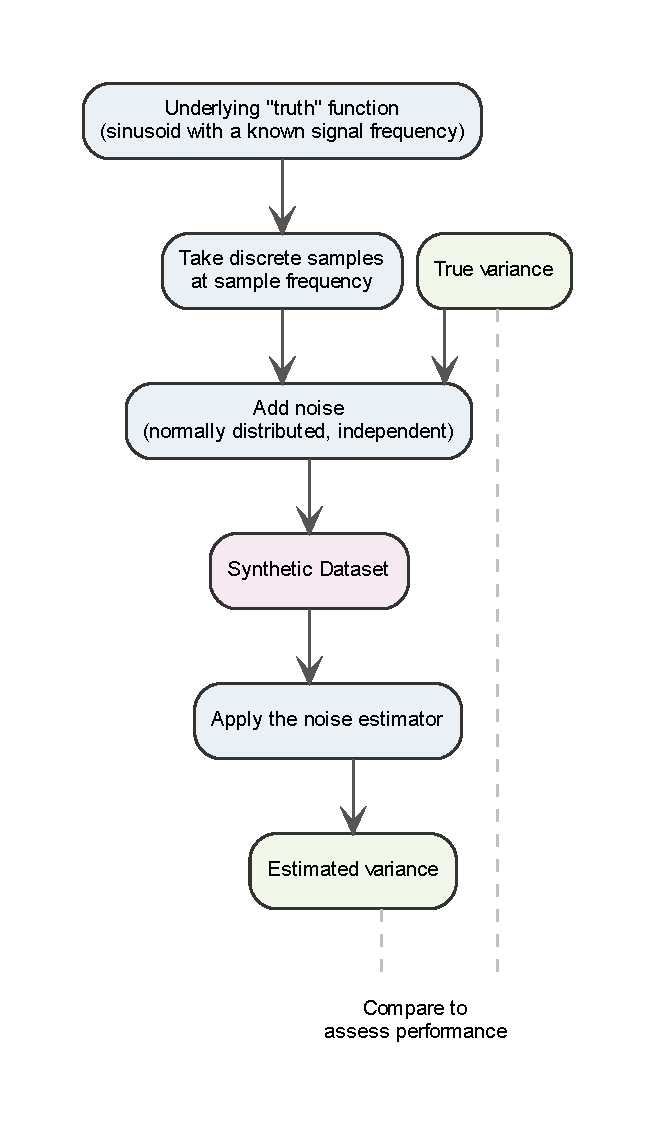
\includegraphics[trim=1cm 1cm 1cm 1cm,clip=true]{../figures/aircraft_sysid/noise_variance_demo_procedure}}
    \caption{Procedure for numerical demonstration of estimator performance}
    \label{fig:noise_variance_demo_procedure}
\end{figure}

As shown in Table \ref{tab:noise_variance_demo}, the first-order noise estimator yields a $\sigma_n$ value that is very close to the true value. We will also show later that this estimator is convergent to the true value as the number of samples increases.

However, this estimator is only first-order convergent with respect to the ratio between the sampling frequency $f_{\rm sample}$ and the underlying dynamics of the system $f_{\rm signal}$. In other words, if the system is ``fast'' relative to the sample rate, then the estimator will be inaccurate. This is demonstrated in the third row of Table \ref{tab:noise_variance_demo}, where the estimator produces an incorrect result by a factor of 3.

\subsubsection{Second-Order Noise Estimator}

To do a better job of estimating the noise variance even in cases where $f_{\rm sample} \gg f_{\rm signal}$ doesn't strictly hold, we can use a second-order estimator. With this extension, we use a three-point numerical stencil.

Derivation of this estimator follows similar principles to the first-order estimator above, with the key result as follows:

\begin{equation}
    \sigma_n^2 = \frac{1}{6 \cdot (N-2)} \sum_{i=1}^{N-2} \Big( x(t_{i+2}) - 2 \cdot x(t_{i+1}) + x(t_i) \Big)^2
    \label{eq:2nd_order_noise_estimator}
\end{equation}

\noindent where $N$ is the number of samples in the dataset. As shown in Table \ref{tab:noise_variance_demo}, the second-order estimator has superior performance to the first-order estimator when the sample and signal frequencies are not well-separated.

Notably, this effectively implements a first-order, second-degree finite-difference of the underlying data—a discrete derivative. It's instructive to consider the theoretical underpinning of using a discrete derivative operator here. If we assume that the underlying true signal is relatively low-frequency (i.e., smooth), then as we take more discrete derivatives of the observed data, the signal component will asymptote to zero (assuming $f_{\rm sample} \geq f_{\rm signal}$). Stated equivalently, the frequency spectrum of the true signal is assumed to have some cutoff frequency (analogous to $f_{\rm signal}$), above which the power spectral density gradually goes to zero.

In contrast, the noise is assumed to be independent, which means that the noise component of the observed data will not go to zero as we take successive derivatives. Stated equivalently, the frequency spectrum of the noise is white, with uniform spectral power across all frequencies. Therefore, repeated application of the discrete derivative operator acts as a way to spectrally-separate the noise from the signal - a key insight into this method.

\subsubsection{Arbitrary-Order Estimators}

Clearly, the second-order estimator improves performance compared to the first-order one. Interestingly, we can generalize the logic to an $d$-th order estimator by observing that the denominator is the sum of the squares of the first-order, $d$-th-degree, uniform-grid finite difference coefficients\footnote{Or, perhaps more intuitively, the elements of the $d$-th row of Pascal's triangle}. Then, we use the combinatorial trick that:

\begin{equation}
{d \choose 0}
    ^2 + {d \choose 1}^2 + \dots + {d \choose d}^2 = {2 d \choose d} = \frac{(2d)!}{(d!)^2}
\end{equation}

\noindent to derive the following $d$-th order estimator of the noise variance:

\begin{equation}
    \sigma_n^2 =
    \frac{1}{{2 d \choose d} \cdot (N-d)}
    \cdot \sum_{i=1}^{N-d} \left[
            {d \choose 0} x(t_i)
        - {d \choose 1} x(t_{i+1})
        + {d \choose 2} x(t_{i+2})
        - {d \choose 3} x(t_{i+3})
        \pm \dots
        \mp {d \choose d} x(t_{i+d})
        \right]^2
    \label{eq:arbitrary_order_noise_estimator}
\end{equation}

Though equation \ref{eq:arbitrary_order_noise_estimator} gives the correct expression for this estimator, numerically implementing this requires some care. Appendix \ref{sec:estimator_code_example} outlines some considerations here and gives an example stable numerical implementation of this estimator.

While we have shown that the second-order estimator has improved robustness to low sample rates, it is not immediately clear that this will hold for arbitrary orders - as the order increases, we might expect to see some form of numerical instability as we take successively higher-order derivatives of noisy data. To test this, we can plot the performance of noise estimators of various orders, as shown in Figure \ref{fig:noise_variance_higher_order}.

\begin{figure}[!htb]
    \centering
    \ifdraft{}{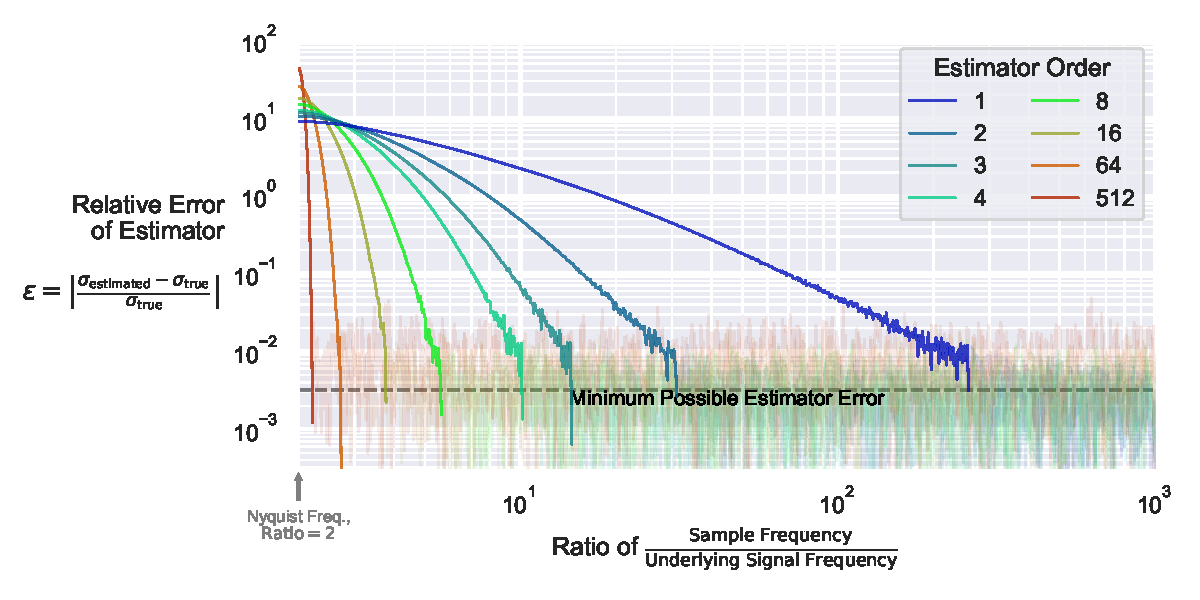
\includegraphics[width=\textwidth]{../figures/aircraft_sysid/noise_variance_higher_order}}
    \caption{Performance of higher-order data-driven noise estimators}
    \label{fig:noise_variance_higher_order}
\end{figure}


The figure above shows something quite remarkable: we can use extremely-high-order estimators (even up to the 512th order, i.e., taking the 512th-derivative of raw, noisy data via finite differences), and we see not only that it's numerically stable, but also that it accurately estimates the true noise variance even when the underlying signal is almost at the Nyquist frequency.

Interestingly, except for a miniscule region near the Nyquist frequency, estimator performance seems to monotonically improve with increasing estimator order. Since practical data reconstruction would likely have the $f_{\rm sample} / f_{\rm signal}$ ratio be much larger than 2, this suggests that one can use extremely-high-order estimators to estimate the noise variance with very high accuracy.

\subsection{Uncertainty Quantification Using Noise Variance Estimators}

With the ability to estimate the amount of noise in the data, we can also estimate the uncertainty of our resulting models and curve fits. To do this, we combine a resampling bootstrap approach (described in \cite{surrogates, elements_of_statistical_learning}) with a noise-variance-aware spline interpolator (described in \cite{surrogates, wahba}). Together, these yield not only a best-estimate of the underlying model, but also a measure of the uncertainty in that estimate. An example is depicted in Figure \ref{fig:power_curve_spline_but_no_physics}, which uses the same power-curve dataset as in Figure \ref{fig:power_curve_naive}.

\begin{figure}[!htb]
    \centering
    \ifdraft{}{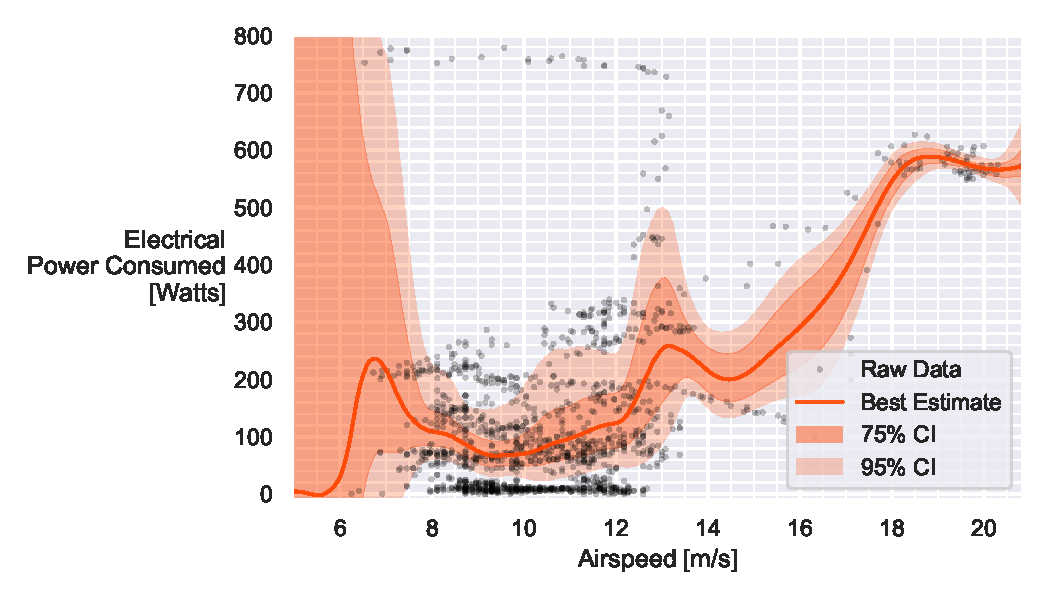
\includegraphics[width=\textwidth]{../figures/aircraft_sysid/power_polar_spline_but_no_physics}}
    \caption{Raw uncorrected data for the power curve, with a noise-variance-aware spline model. A resampling bootstrap allows uncertainty quantification. This improves over the naive approach of Figure \ref{fig:power_curve_naive}, although, the lack of physics-based model structure still leads to the recovery of a physically-implausible result.}
    \label{fig:power_curve_spline_but_no_physics}
\end{figure}

Figure \ref{fig:power_curve_spline_but_no_physics} certainly represents an improvement over the naive curve fits shown in Figure \ref{fig:power_curve_naive} in that it leverages uncertainty. For example, the uncertainty narrows near $19\ \rm m/s$ where data is abundant, and it widens considerably below $7\ \rm m/s$ where data is sparse. This awareness of model uncertainty reduces our propensity to make statistical conclusions that go beyond what the data can truly support.

Furthermore, this uncertainty quantification allows us to determine where in the flight envelope more data should be collected (i.e., serve as an acquisition function). For example, to refine the power curve of Figure \ref{fig:power_curve_spline_but_no_physics}, we might aim to fly future test flights at speeds between 13 and 17 m/s.

With this said, two major problems remain with the approach of Figure \ref{fig:power_curve_spline_but_no_physics}. First, the resulting model uncertainty is extremely high, as shown by the shaded confidence intervals in Figure \ref{fig:power_curve_spline_but_no_physics}. For example, the tightest that we can bound the required power at $10\ \rm m/s$ with reasonably-strong confidence (95\% confidence interval) is between $30$ and $190$ Watts. This is a huge range and not a particularly useful insight. Near the low end of the airspeed range, the model uncertainty becomes so large that even the most basic claims are impossible to assert.

Second, the model still allows physically-implausible relationships, such as the unexplained power curve increase near $13\ \rm m/s$ and the flattening power curve near $20\ \rm m/s$. Clearly, the uncertainty bounds here are wider than what they would be if our physical insights were incorporated into the model.


\section{Incorporating Physics-Based Data Corrections and Domain-Specific Knowledge}
\label{sec:physics_based_corrections}

When inferring the performance characteristics of a physical system, the laws governing that system can be used to significantly narrow the solution space and reduce the unexplainable variance in the data.

\subsection{The Aircraft as an Energy System}

In the example of the power curve regression, one way to do this is to consider the aircraft as an energy system and exploit the fact that energy should be conserved. Consider the following basic accounting equation for the total energy of an aircraft at some time $t$:

\begin{equation}
    E_{\rm total}(t) =
    \frac{1}{2}m \, U(t)^2
    + m \, g \, h(t)
    + \int_0^t \left[
        P_{\rm loss}(\tau)
        - P_{\rm thrust}(\tau)
        \right] \, d\tau = \text{constant}
    \label{eq:total_energy}
\end{equation}

\begin{eqexpl}
    \item{$E_{\rm total}$} Total energy of the aircraft system. System boundary includes the aircraft but not the onboard stored energy (e.g., battery) or power-to-air (e.g., drag); hence, the representation of these as flow terms. Sign convention is that energy added to the airplane is positive.
    \item{$m$} Mass of the aircraft
    \item{$U(t)$} Airspeed of the aircraft at time $t$
    \item{$g$} Local gravitational acceleration
    \item{$h(t)$} Altitude of the aircraft at time $t$
    \item{$P_{\rm thrust}(t)$} Thrust power ($T \cdot U$) to the aircraft at time $t$
    \item{$P_{\rm loss}(t)$} Power lost from the aircraft at time $t$; primarily drag, but also other system losses
\end{eqexpl}

\noindent Note that the above equation is ``fully-accounted'' in that it includes all energy flows into and out of the airplane, including from onboard sources. Hence, $E_{\rm total}$ should remain constant throughout the flight.

To exploit this knowledge that $E_{\rm total}$ is constant, we differentiate Equation \ref{eq:total_energy} with respect to time to obtain an expression for the total power. The total power must equal zero for energy conservation to hold. In writing the following expression, we can also expand the power gains and losses into constituent terms as appropriate for an electric aircraft:

\begin{equation}
    P_{\rm total}(t) =
    m \, U(t) \, \dot{U}(t)
    + m \, g \, \dot{h}(t)
    + \left[
        U(t) \, D(\theta)
        + P_{\rm avionics}
        - V(t) \, i(t) \, \eta_{\rm propulsive}(\theta)
        \right] = 0
    \label{eq:total_power}
\end{equation}

\begin{eqexpl}
    \item {$\dot{(\:)}$} Time derivative
    \item {$P_{\rm total}(t)$} Total power at time $t$. Just as with $E_{\rm total}$, this is a ``fully-accounted'' quantity, and hence $P_{\rm total}$ should equal zero.
    \item {$V(t)$} Battery voltage at time $t$
    \item {$i(t)$} Battery current at time $t$
    \item {$\eta_{\rm propulsive}(\theta)$} Propulsive efficiency ($P_{\rm thrust} / P_{\rm in}$) as a function of both flight data and unknown parameters $\theta$
    \item {$P_{\rm avionics}$} Power consumed by avionics. In the case of the example dataset, this is assumed to be constant and equal to the average measured power consumption during motor-off periods.
    \item {$D(\theta)$} Drag as a function of both flight data and unknown parameters $\theta$
\end{eqexpl}

Ideally, this equation would be used to simply correct the data for the unsteady terms (i.e., acceleration and climb terms) in Equation \ref{eq:total_power}, at which point we would directly use that data and apply traditional curve-fitting techniques. However, the observant reader will notice that Equation \ref{eq:total_power} cannot, on its own, be used to correct the data. Both the propulsive efficiency and drag terms are unknown functions of the flight data and unknown parameters $\theta$, and hence these need to be solved for.

These parameters can be defined as the solution of a residual minimization problem (i.e., optimization) between our data and model—effectively, system identification. Here, the residual in question is the instantaneous $P_{\rm total}$ given in Equation \ref{eq:total_power}, and we aim to minimize some norm\footnote{Typically the $L_1$ or $L_2$ norm} of the residual vector, as resampled from the data reconstruction shown in Section \ref{subsec:optimal_sensor_data_reconstruction}. However, the interesting insight here is that changes to our model parameters affect \emph{both} the model and the corrected data, and hence the model and data must be optimized simultaneously. Stated equivalently: we are not only correcting the data using our models; we are also simultaneously fitting the models to the data.

One other consideration to note with this energy-corrected formulation is that it relies on the time derivative of sensor data. Because our data reconstructors from Section \ref{subsec:optimal_sensor_data_reconstruction} are based on splines, these can be conveniently differentiated by conducting simple polynomial differentiation piecewise between knot points. However, the derivative of the best estimator is not necessarily the bias-variance-optimal estimator of the derivative, due to the amplification of high-frequency variation during the differentiation process. To combat this, we add a Gaussian low-pass-filter with time constant $\sigma=4\ \rm sec$ to the derivative estimator. Developing a rigorous method for determining the optimal filter time constant is left as future work, but is theoretically possible using a cross-validation approach.

\subsection{Modeling the Unknown Functions}
\label{subsec:modeling_unknown_functions}

There are two unknown models in Equation \ref{eq:total_power}: the propulsive efficiency and the drag. We replace these with parametric models with forms taken from domain-specific knowledge. In this example, we use simple mathematical relations to demonstrate that even basic restrictions on model form can significantly improve the quality of the resulting model. In practice, more sophisticated models based on parameterized low-fidelity analyses could be used, although this may come at the expense of reduced interpretability.

\subsubsection{Drag Model}
\label{subsubsec:drag_model}
The aerodynamic drag can be modeled as a function of airspeed, as required to close Equation \ref{eq:total_power}. To do this, we use the following procedure:

\begin{enumerate}
    \item Compute the instantaneous lift coefficient $C_L(t)$ from the airspeed $U(t)$, assuming a load factor of 1 and known aircraft properties (wing area, mass, etc.).
    \item Map the $C_L$ to a drag coefficient $C_D$ using a parametric model with unknown parameters $\theta_1$ to $\theta_6$. The form of this model is a piecewise-quadratic $C_D(C_L)$ function, as shown in Figure \ref{fig:aero_polar_form}. This model form is identical to the assumed form of the profile drag function in the AVL \cite{drela_athena_2004} aerodynamics code. In this model form:\\
    \begin{itemize}
        \item $(\theta_1, \theta_2)$ represents the point of positive stall onset
        \item $(\theta_3, \theta_4)$ represents the minimum drag point
        \item $(\theta_5, \theta_6)$ represents the point of negative stall onset
    \end{itemize}
    \ \\The piecewise-quadratic function is constructed to be $C^1$-continuous between the four regions delineated by these points. This requirement fully-constrains the non-stalled regions of the curve. The regions above positive stall and below negative stall use an assumed curvature (identical to the values used in AVL \cite{drela_athena_2004}) that generally models post-stall drag rise.

    \item Dimensionalize the computed $C_D$ to obtain the drag.
\end{enumerate}

\begin{figure}[h]
    \centering
    \includesvg{../figures/aircraft_sysid/aero_polar_form.svg}
    \caption{Assumed parameterized form of the aerodynamic polar, where drag coefficient is a piecewise-quadratic function of the lift coefficient. Same mathematical form as the profile drag function used by AVL \cite{drela_athena_2004}.}
    \label{fig:aero_polar_form}
\end{figure}

\subsubsection{Propulsive Efficiency Model}
\label{subsubsec:propulsive_efficiency_model}

Similarly, a characteristic model for the propulsive efficiency is defined based on domain-specific knowledge. In an ideal case, this model would take the propeller advance ratio $J$ as an input and yield the propulsive efficiency $\eta_{\rm propulsive}$ as an output. However, the advance ratio is not directly measurable in this \emph{Solar Surfer} case study, as this requires propeller RPM data which is not available. However, we do have sufficient data to infer a quantity known to differ from the advance ratio $J$ by a constant factor; we denote this proportional quantity $c_J$.

Therefore, the propulsive efficiency model is a mapping from $c_J$ to $\eta_{\rm propulsive}$, rather than from $J$ to $\eta_{\rm propulsive}$. Although this means that the maximum-efficiency advance ratio $J$ cannot be estimated, the peak propulsive efficiency itself can be estimated; ultimately, it is the peak efficiency that is the primary performance metric of interest.

To construct this model, we use the following procedure:

\begin{enumerate}
    \item Use the measured current $i(t)$ to estimate $c_n$, a quantity proportional to the propeller rotational rate $n$, using the $P_{\rm in}\propto n^3$ relationship found using the Buckingham $\pi$ theorem \cite{unified_propellers}:
    \begin{equation*}
        c_n = i(t)^{1/3} \propto n
    \end{equation*}
    \item Propagate this to estimate $c_J$, a quantity proportional to the propeller advance ratio $J$:
    \begin{equation*}
        c_J = \frac{U(t)}{c_n} \propto J
    \end{equation*}
    \item Map $c_J$ to a propulsive efficiency $\eta_{\rm propulsive}$ using the following model form and unknown parameters $\theta$:

    \begin{equation}
        \eta_{\rm propulsive} =
        \theta_7 \cdot \text{softmin} \left(\
        c_J / \theta_8,\quad
        \frac{c_J - \theta_9}{\theta_8 - \theta_9}\
        \right)
    \end{equation}

    \noindent where softmin is a smooth approximation of the minimum function, analogous to the logsumexp definition of softmax by Cook and others \cite{cook_basic_2011}:

    \begin{equation*}
        \text{softmin}(x, y) = -\theta_{10} \cdot \ln \left( e^{-x / \theta_{10}} + e^{-y / \theta_{10}} \right)
    \end{equation*}
%        where all parameters $\theta_i$ here are constrained in such a way that $0 \leq \eta_{\rm propulsive} \leq 1$ always.

    \noindent Note the physical interpretation of several parameters here:
    \begin{itemize}
        \item $\theta_7$ provides an upper bound on the peak propulsive efficiency
        \item $\theta_8$ represents the $c_J$ value corresponding to peak efficiency
        \item $\theta_9$ represents the $c_J$ value corresponding to the ``pitch speed'' of the propeller, where the thrust (and hence efficiency) goes to zero.
        \item $\theta_{10}$ is a smoothing parameter that controls the sharpness of the transition between the two regions.
    \end{itemize}\ \\
    \noindent This model form captures expected behavior of the propulsive efficiency curve, including the fact that the propulsive efficiency is zero at zero airspeed and zero at the pitch speed of the propeller. The $\theta_7$ parameter is constrained to be less than one to bound efficiency to physically-plausible values. The resulting model form matches well with expected propeller efficiency trends, such as the curves seen in \cite{unified_propellers}.
\end{enumerate}

\subsection{Solving the Optimization Problem}
\label{subsec:solving_optimization_problem}

With these models in place, a residual minimization problem of the following form can be solved to yield optimal $\theta$ values, where $P_{\rm total}$ (the net power into the system, after all inflows and outflows should be accounted for) from Equation \ref{eq:total_power} is used as the residual:

\begin{mini}
    |l|
        {\theta}{\sum (P_{\rm total})^2}
        {}{}
    \addConstraint{\theta\ \text{constraints described in Section \ref{subsec:modeling_unknown_functions}}}
    \label{eq:}
\end{mini}

Optionally, other norms of the $P_{\rm total}$ residual vector can be minimized instead. The $L_1$ norm makes a particularly compelling choice here due to its robustness to outliers \cite{brunton_data_2017}. In the example problem here, we solve this optimization problem numerically using IPOPT \cite{ipopt} via the AeroSandbox \cite{sharpe_aerosandbox_2021} framework for engineering design optimization.

\subsection{Results}

With the optimization problem solved, we can now use the resulting $\theta$ values to compute the corrected data and model. This is shown in Figure \ref{fig:power_curve_with_physics}. The corrected data and model are now in excellent agreement, and the corrected data has significantly less unexplained variance than the raw data. The remaining unexplained variance is attributable to a variety of factors, such as wind updrafts and downdrafts and non-unity load factors during banked flight. In theory, both these effects could be corrected out using a similar inference procedure that is shown in this work (which could be augmented by, for example, IMU data). This is left as future work, which, if successful, would reduce the data spread in Figure \ref{fig:power_curve_with_physics} further.

\begin{figure}[!htb]
    \centering
    \ifdraft{}{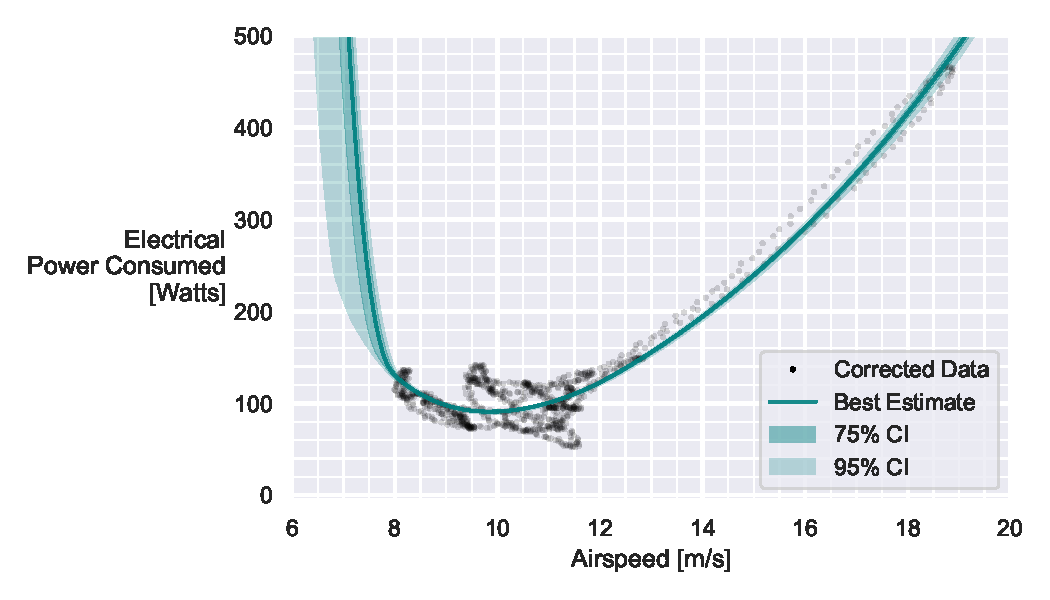
\includegraphics[width=\textwidth]{../figures/aircraft_sysid/power_curve_with_physics.pdf}}
    \caption{Inferred power curve with physics-informed corrections on data and model, and using noise estimator with a resampling bootstrap for uncertainty quantification. Power curve agrees closely with the data and shows physically-plausible behavior. Uncertainty quantification is significantly tighter than in Figure \ref{fig:power_curve_spline_but_no_physics}, as the function space has been restricted using embedded physics knowledge.}
    \label{fig:power_curve_with_physics}
\end{figure}

Conveniently, this process yields other critical performance information, like the aerodynamic polar and propulsive efficiency curve, ``for free'' as part of the fitting process. These are shown in Figures \ref{fig:aerodynamic_polar_with_physics} and \ref{fig:propeller_polar_with_physics}. Furthermore, we also obtain uncertainty estimates for all these quantities, which are critical for understanding the confidence we can have in the results.

A notable observation is that the inferred aerodynamic polar of Figure \ref{fig:aerodynamic_polar_with_physics} and the propulsive efficiency curve of Figure \ref{fig:propeller_polar_with_physics} show relatively wide uncertainty bands, while the power curve of Figure \ref{fig:power_curve_with_physics} shows a relatively narrow uncertainty band. This is interesting, since in typical analysis the power curve is computed as a function of these two performance relations; hence, one would intuitively expect that the power curve would inherit the uncertainty of both relations. The reason this does not occur here is that the uncertainties in the aerodynamic polar and the propulsive efficiency curves are not independent. In other words, the power required can be inferred relatively precisely, but there is not quite enough data to rigorously determine whether power losses are more due to aerodynamic drag or propulsive inefficiency.

\begin{figure}[!htb]
    \centering
    \ifdraft{}{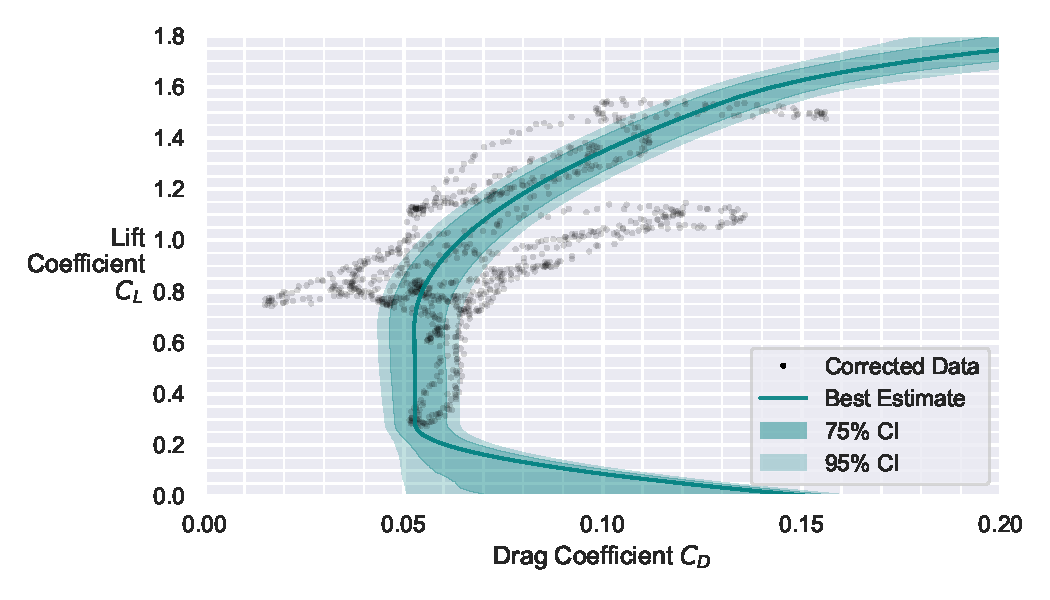
\includegraphics[width=\textwidth]{../figures/aircraft_sysid/aerodynamic_polar_with_physics.pdf}}
    \caption{Inferred aerodynamic polar with physics-informed corrections on data and model, and using noise estimator with a resampling bootstrap for uncertainty quantification.}
    \label{fig:aerodynamic_polar_with_physics}
\end{figure}

Compared to the naive approach in Figure \ref{fig:power_curve_naive}, Figure \ref{fig:power_curve_with_physics} enables us to make very accurate, physically-grounded, and uncertainty-quantified assertions about the performance of the airplane, based on minimal data (here, only four minutes of flight time).

\begin{figure}[!htb]
    \centering
    \ifdraft{}{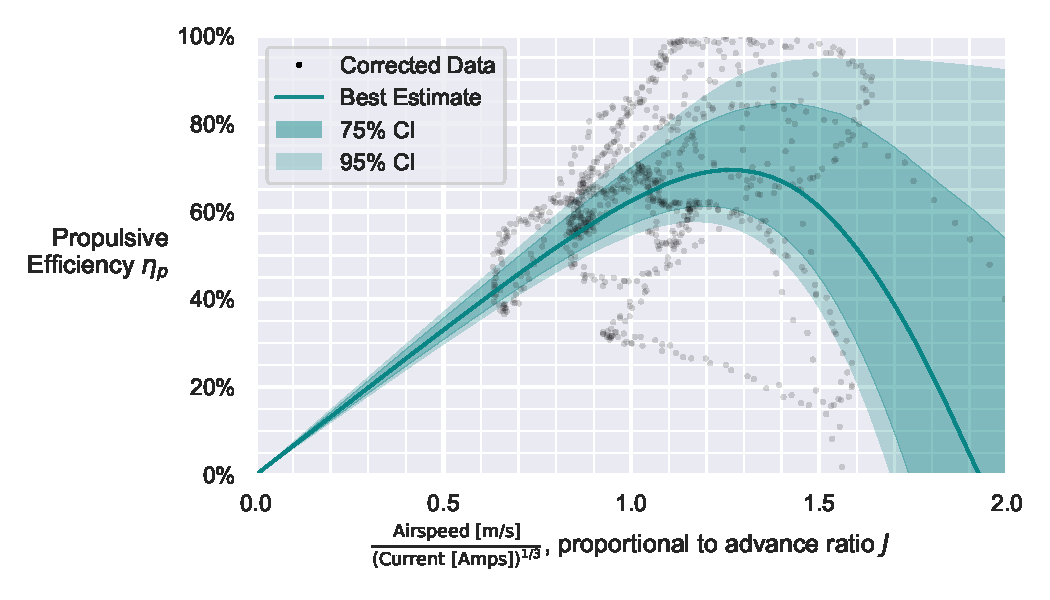
\includegraphics[width=\textwidth]{../figures/aircraft_sysid/propeller_polar_with_physics.pdf}}
    \caption{Inferred propulsive efficiency curve with physics-informed corrections on data and model, and using noise estimator with a resampling bootstrap for uncertainty quantification.}
    \label{fig:propeller_polar_with_physics}
\end{figure}


\section{Computational Reproducibility}

All code and data used in this chapter is publicly available at \url{https://github.com/peterdsharpe/aircraft-polar-reconstruction-from-flight-test}.


\section{Summary and Future Work}
\label{sec:sysid_conclusion}

In this chapter, we have demonstrated a rigorous method for reconstructing the performance characteristics of an aircraft from flight test data. This method is based on a physics-informed correction of the data and model, and is shown to be effective at recovering the true power curve and aerodynamic polar of an example aircraft from noisy, limited, unsteady data. This method is also shown to be robust to the presence of outliers in the data, and to be able to provide uncertainty estimates for the resulting aerodynamic polar. This method is also shown to be able to recover the propulsive efficiency curve of the aircraft, which is a critical quantity for understanding the performance of the aircraft. Finally, this method is shown to be able to recover the aerodynamic polar of the aircraft from only four minutes of flight test data, which is a significant reduction in the amount of data required compared to the state of the art.

This work has focused on the ability of these inference-based reconstruction procedures to significantly reduce the required flight hours to characterize an airplane's performance. However, an alternative way to ``spend'' this increased ability to extract information is on massively reducing instrumentation costs. For example, this approach makes it conceivable to ``estimate out'' the ambient wind field\footnote{An intuitive explanation for this is that if an airplane loiters in a circle at constant power setting, the upwind and downwind groundspeeds yield information about the wind field. In practice, some additional assumptions about wind steadiness and uniformity would likely be required to collapse the $(x, y, z, t)$ space; otherwise, it is likely too large to realistically span.} from groundspeed data and power measurement alone. If this is possible, it would enable flight test engineers to perform sufficient early-stage characterization of a new crewed airplane using nothing other than the sensors available on a modern smartphone. Here, GPS, IMU, and barometer sensors provide position and groundspeed information, and the phone's microphone can be used to infer engine RPM and hence power and advance ratio from an audio spectrum. If successful, this would be an enormous reduction in instrumentation cost and time compared to the state of the art.

A fair point of hesitancy here might be the fact that applying these corrections to recover useful insights from noisy, limited, unsteady data takes a significant amount of algorithmic development and mathematical complexity. However, algorithms are cheap, and more importantly, scalable - so, once a computational chapterflow is established, it can easily be applied to a large number of flight test campaigns. By contrast, flight-test hours and improved instrumentation represent a recurring high cost. Therefore, it is worth investing in the development of algorithms that can extract the maximum amount of useful insight from the data that we do collect, even if this analysis is somewhat less simple.



%
%\subsection{Solar Surfer Design Drawing}
%\label{sec:solar_surfer_drawing}
%
%\begin{figure}[H]
%    \centering
%    \ifdraft{}{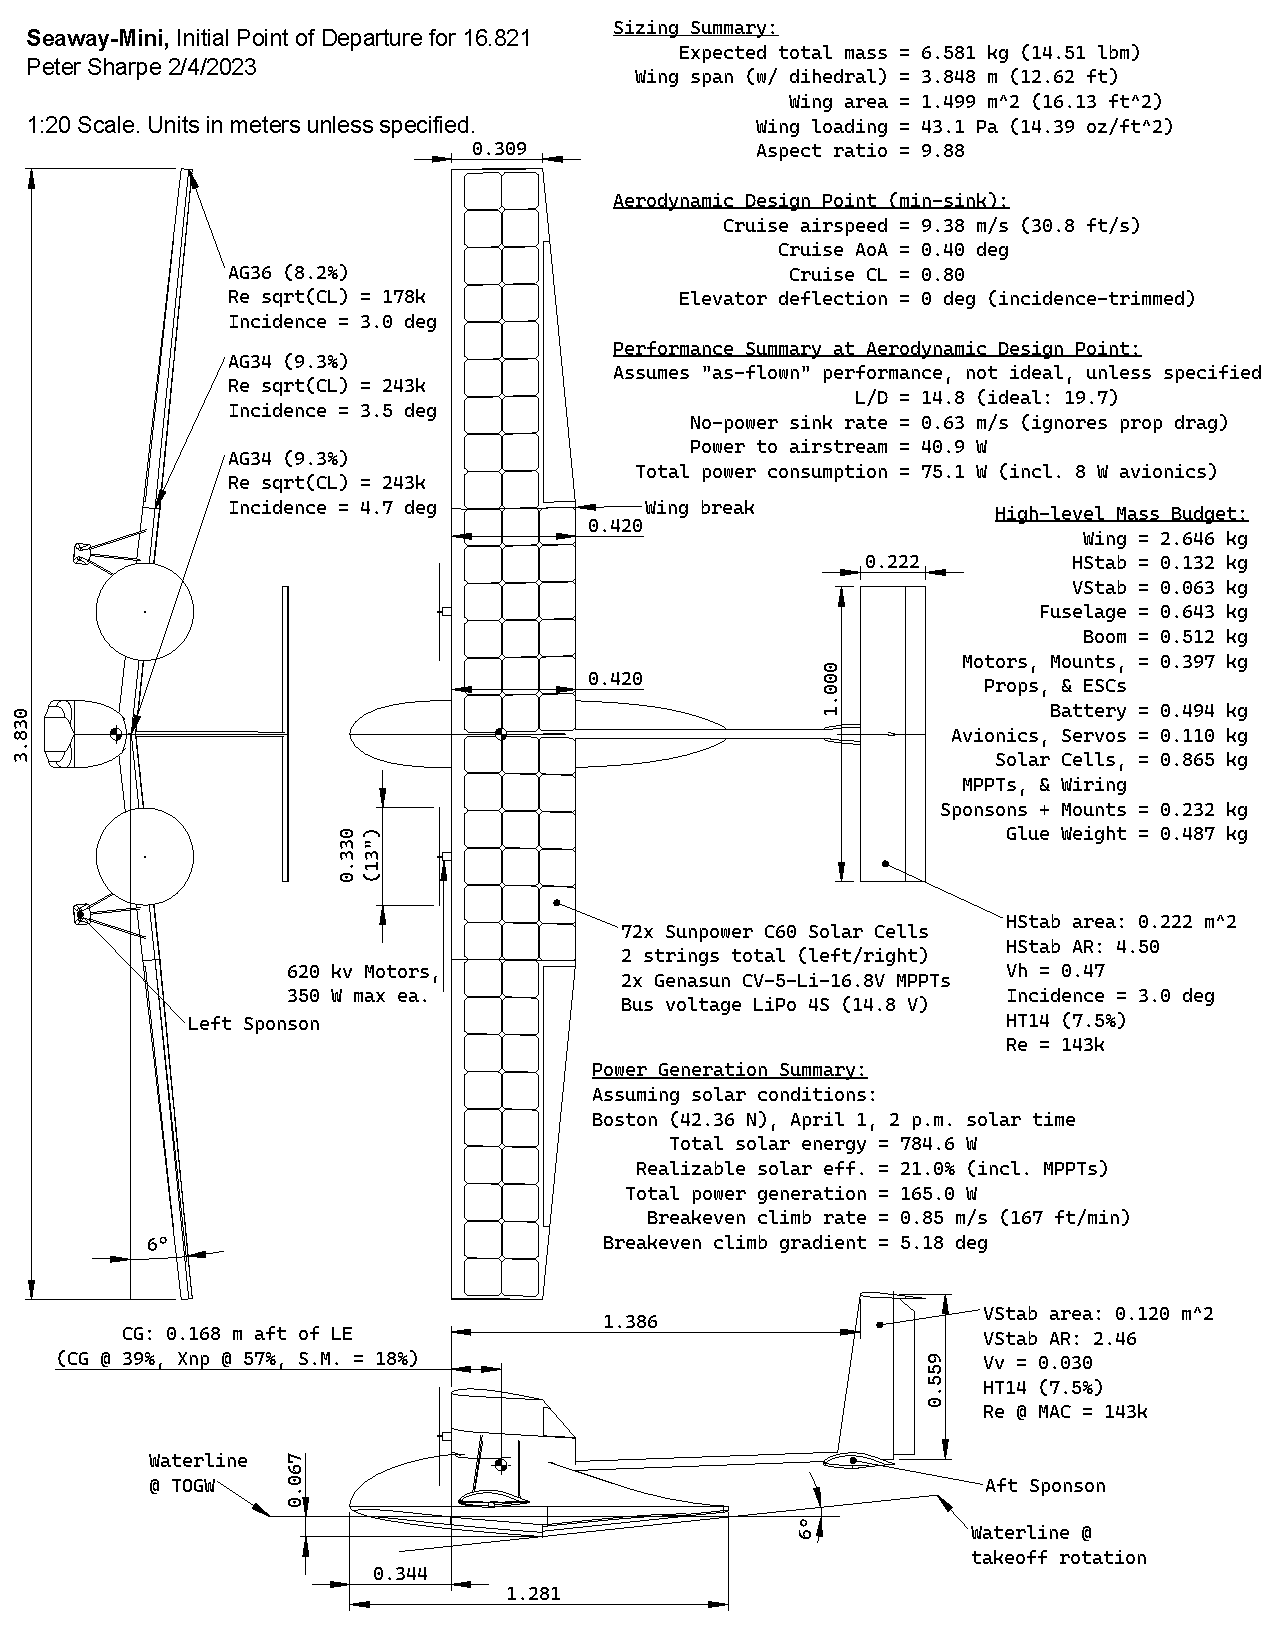
\includegraphics[page=1, width=\textwidth]{../figures/aircraft_sysid/seaway_mini_packet.pdf}}
%    \label{fig:solar_surfer_design}
%\end{figure}

\section*{Chapter Acknowledgments}
The authors would like to thank the MIT AeroAstro 16.821 course staff for their support of the work in this chapter, and the MIT AeroAstro department for their support of the course. The aircraft used to collect the example data in this chapter was constructed by the MIT AeroAstro 16.821 undergraduate student team.

%    \bibliography{main, C:/Users/peter/Documents/Zotero/library, C:/Users/peter/Documents/Zotero/library-zotero}
